
Wie im vorherigen Kapitel beschrieben, existieren verschiedene Varianten, einen \gc Tausch 
durchzuführen. Für das Finden der gemeinsamen Nachbarschaft betrachten wir sieben verschiedene Methoden, 
für das Tauschen der Nachbarschaft zwei und weiterhin prüfen wir noch, ob es sinnvoll ist, 
die \red{vorsortiert} Invariante zu nutzen oder nicht, was ebenfalls zwei Möglichkeiten entspricht.
Kombiniert man all diese Möglichkeiten erhält man also insgesamt 28 verschiedene Varianten für einen \gc 
Tausch.
In diesem Kapitel diskutieren wir, welche der Varianten ausgewählt wurde.
%%%%%%%%%%%%%%%%%%%%%%%%%%%%%%%%%%%%%%%%%%%%%%%%%%%%%%%%%%%%%%%%%%%%%%%%
%%%%%% Aufbau
%%%%%%%%%%%%%%%%%%%%%%%%%%%%%%%%%%%%%%%%%%%%%%%%%%%%%%%%%%%%%%%%%%%%%%%%

\section{Versuchsaufbau}
Um die einzelnen Varianten auf Ihre Laufzeit zu testen, wurde eine Art Versuch aufgebaut.
Dazu wurden alle Methoden in \cpp programmiert. Diese wurden dann auf unterschiedlichen
Instanzen getestet und mittels Google Benchmark \cite{benchmark} wurde die Zeit gemessen, 
die für das Ausführen benötigt wurde.
\\
\\
\red{Google Benchmark ist ein \red{Framework} ...?}
\\
\\
Wie %\red{vorher (kapitel ..?)} 
beschrieben benötigen die Methoden als Eingabe keinen Graph, 
sondern lediglich zwei Vektoren, welche jeweils die Nachbarschaft zweier Knoten repräsentieren. Ohne 
Beschränkung der Allgemeinheit nennen wir den größeren (sofern einer der beiden Vektoren größer ist)
$u$ und den kleineren $v$.
Um möglichst gut zu erkennen, wie sich die verschiedenen Methoden bei unterschiedlichen
Eingaben verhalten, messen wir die Laufzeiten für eine ganze Reihe an Instanzen. 
Um ein gutes Bild zu erhalten, sollten folgende Fälle auf jeden Fall abgedeckt sein:

\begin{itemize}
	\item Beide Vektoren liegen in der gleichen Größenordnung
	
	\item Einer der Vektoren ist wesentlich größer als der andere
	
	\item Der Anteil an gemeinsamen Nachbarn ist groß
	
	\item Der Anteil an gemeinsame Nachbarn  ist klein
\end{itemize}
Um dies zu erreichen, \red{erstellen} wir mehrere Runden, in denen der Vektor $u$ von anfänglich 128
Elementen auf bis zu 4.000.000 Elementen vergrößert wird. Innerhalb jeder Runde werden mehrere Durchläufe 
durchgeführt, bei denen der Vektor $u$ eine Größe zwischen 32 Elementen und der jeweiligen Größe von $v$ hat.
Für jeden dieser Durchgänge werden die beiden Vektoren mit zufälligen, aber paarweise verschiedenen,
Werten befüllt, bis sie die entsprechende Größe haben. 
Dabei haben die Vektoren aber offensichtlich keine Elemente gemeinsam, was dazu führen würde, dass ein \gc 
Tausch nichts verändern würde. Um sicherzugehen,
dass die gemeinsamen Nachbarschaft nicht leer ist, müssen somit Elemente des einen Vektors 
in den anderen hineinkopiert werden. Damit die Größe der gemeinsamen Nachbarschaft
variiert wird, werden zuerst 10, dann 25, 50 und 75 Prozent der Elemente kopiert. 
\\
Eine einzelne Test Messung sich also durch das Tupel \fett{(large, small, fraction)} beschreiben, wobei
\fett{\la} die Größe von $u$ ist, \fett{\sm} die Größe von $v$ und \fett{\fr} der Anteil der gemeinsamen Elemente.
Um eventuelle Messfehler zu minimieren, wird jeder Durchlauf durch Google Benchmark 5 mal wiederholt.
\\
\\
Alle Messungen wurden \red{auf einem Rechner} mit \red{63GB} Arbeitsspeicher und 16 Prozessoren vom Typ Intel(R) Xeon(R) CPU E5-2630 v3 @ 2.40GHz,
welche jeweils 8 Kerne und einen Cache von 20 MB haben, ausgeführt.
\
\\
\\
\red{benchmark mintime..?}
\\
\red{WIE WERDEN DIE Varianten BEZEICHNET..?}
\\
\\
\red{mit hilfe von Jupyter notebook ausgewertet... daten aus json file }
%%%%%%%%%%%%%%%%%%%%%%%%%%%%%%%%%%%%%%%%%%%%%%%%%%%%%%%%%%%%%%%%%%%%%%%%
%%%%%% Global Curveball
%%%%%%%%%%%%%%%%%%%%%%%%%%%%%%%%%%%%%%%%%%%%%%%%%%%%%%%%%%%%%%%%%%%%%%%%

\section{Messung}

Insgesamt wurde für 672 Instanzen die Laufzeit der einzelnen Methoden gemessen. Die gesamte Dauer
hat dabei  ungefähr 19 Stunden betragen. Die Varianten werden mit einem Tripel bezeichnet,
wobei 
\begin{figure}[h]
\centering
	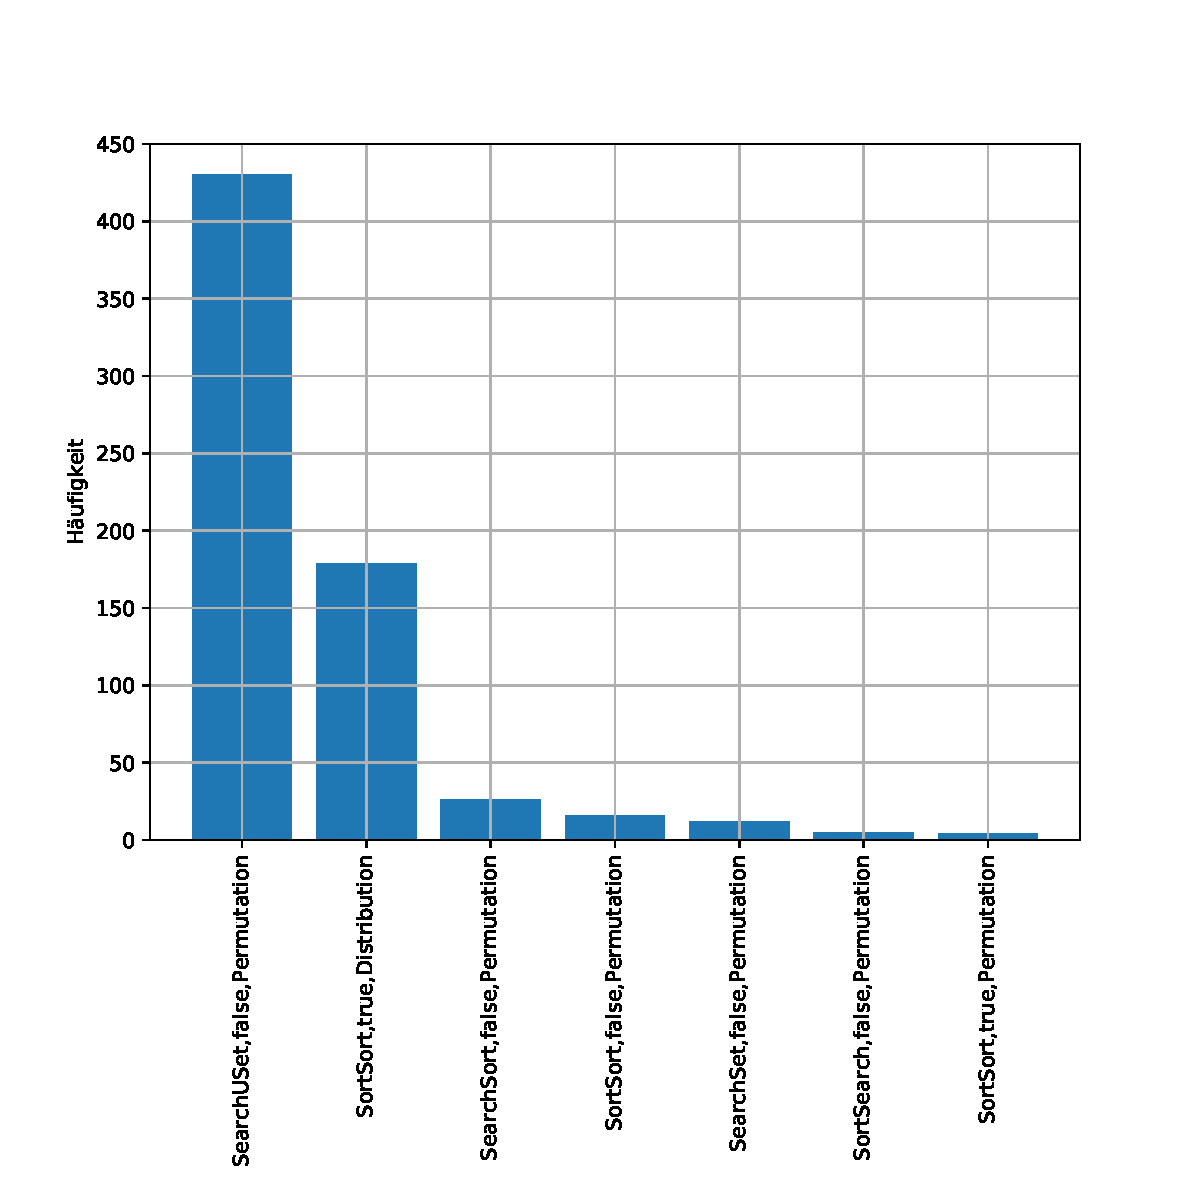
\includegraphics[width = \textwidth]{figures/counting.pdf}
	\caption{\red{Häufigkeit}}
	\label{fig:messung_counting}
\end{figure}
In Abbildung \ref{fig:messung_counting} ist ein Balkendiagramm gegeben, was anzeigt, welche Methoden
pro Instanz am häufigsten die schnellsten sind. Dabei sieht man eindeutig, dass die Variante (\SeaUSet,
false,\perm) mit Abstand auf den meisten Instanzen die schnellste Laufzeit aller Methoden hat. Die
430 Instanzen, auf denen (\SeaUSet,false,\perm) die schnellste Methode ist, entsprechen einem Anteil von rund
64\%. Mit 179 ''gewonnenen'' Instanzen folgt die Variante (\SorSor,true,\distr), was einem Anteil von
27\% entspricht. Zusammen ist somit in etwa 91\% aller getesteter Instanzen eine dieser beiden Methoden
die schnellste gewesen.


\red{\Large wie ist die laufzeit von sortsort, in den instanzen wo das andere gewinnt?? vielleicht ist es ja nicht viel langsamer....}
\begin{figure}[h]
\centering
	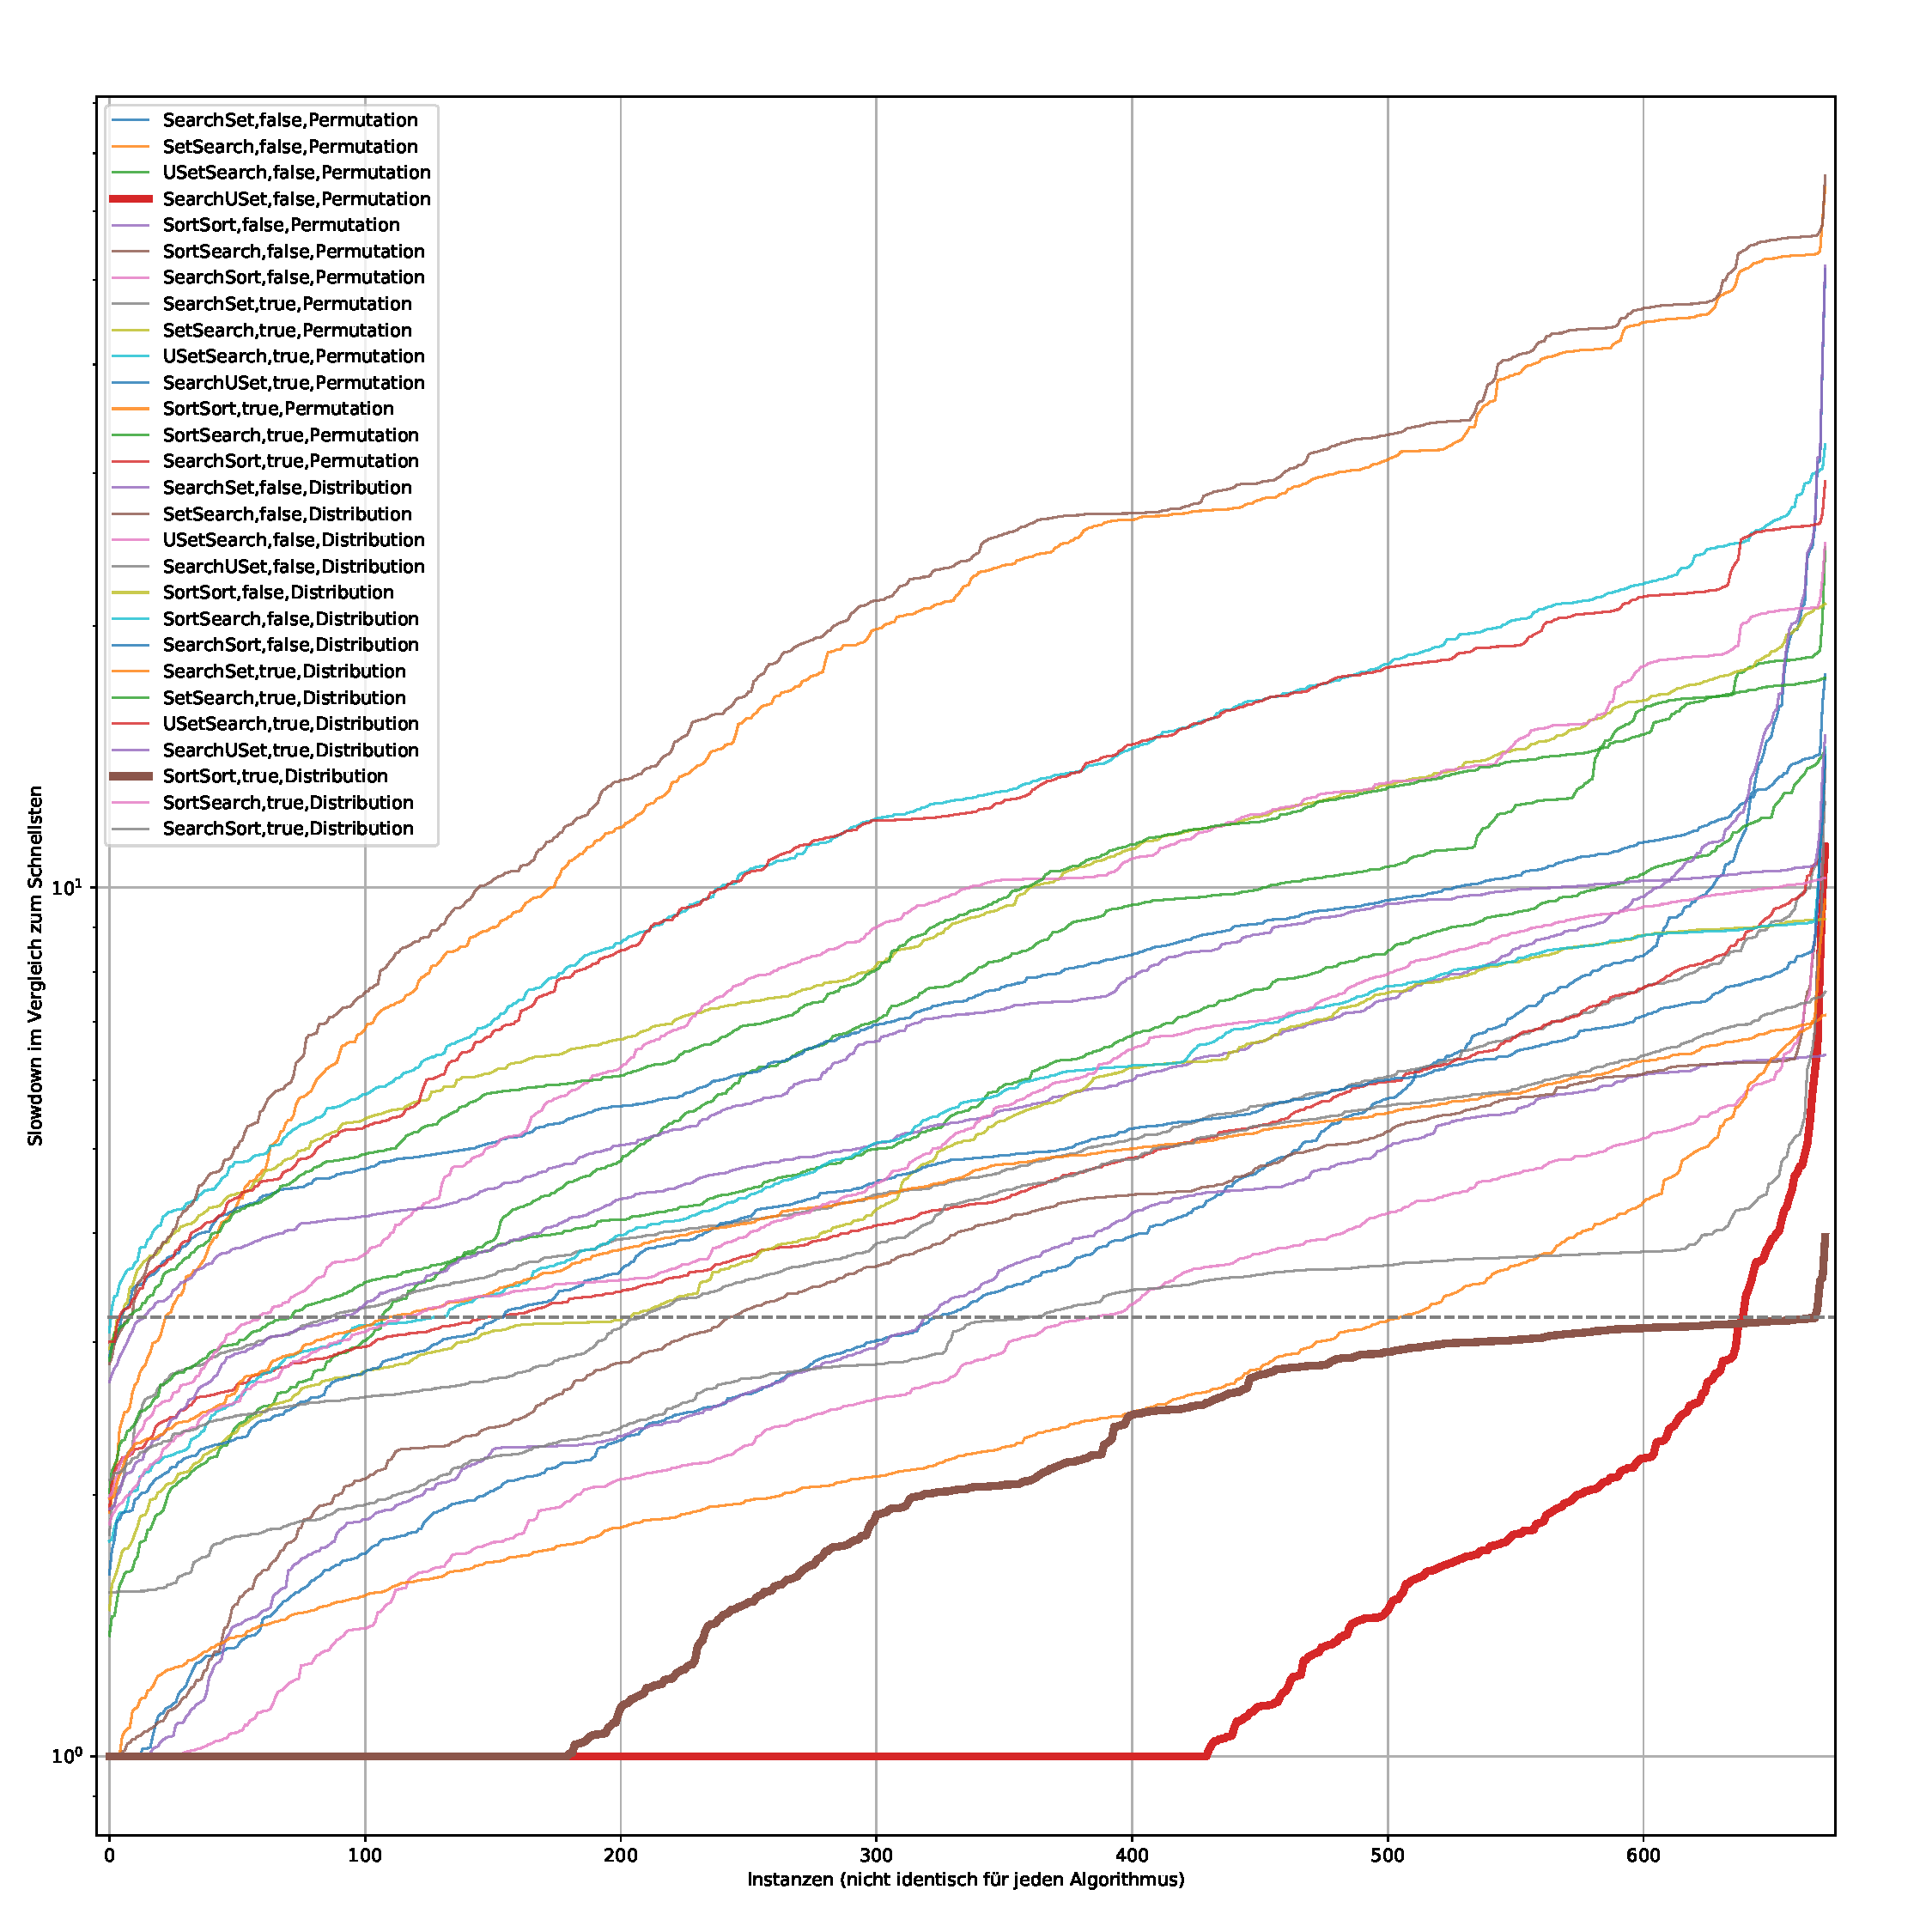
\includegraphics[width = 0.8\textwidth]{figures/slowdown.pdf}
	\caption{Slowdown}
	\label{fig:messung_slowdown}
\end{figure}



%%%%%%%%%%%%%%%%%%%%%%%%%%%%%%%%%%%%%%%%%%%%%%%%%%%%%%%%%%%%%%%%%%%%%%%%
%%%%%% Auswertung
%%%%%%%%%%%%%%%%%%%%%%%%%%%%%%%%%%%%%%%%%%%%%%%%%%%%%%%%%%%%%%%%%%%%%%%%

\section{Auswertung}
